\documentclass[journal,12pt,two column]{IEEEtran}
\usepackage{setspace}
\usepackage{enumitem}
\usepackage[cmex10]{amsmath}
\usepackage{tfrupee}
\usepackage{amsthm}
\usepackage[utf8]{inputenc}
\usepackage{graphicx}
\usepackage{mathtools}
\title{ASSIGNMENT 1 }
\author{Muskan Jaiswal - cs21btech11037}
\newcommand{\solution}{\noindent \textbf{Solution: }}
\begin{document}
\maketitle
\textbf{Problem 1(b):} Solve the equation $4x^2-5x-3=0$ and give your answer correct to 2 decimal places
\\

\textbf{SOLUTION:}     For any kind of equation of the form  $ax^2+bx+c=0$

It's roots are
\\

\begin{align*}
x={\frac{-b\pm\sqrt{b^2-4ac}}{2a}}\\
\end{align*}

For the given equation-
\begin{align}
    4x^2-5x-3=&0
\end{align}
\begin{figure}
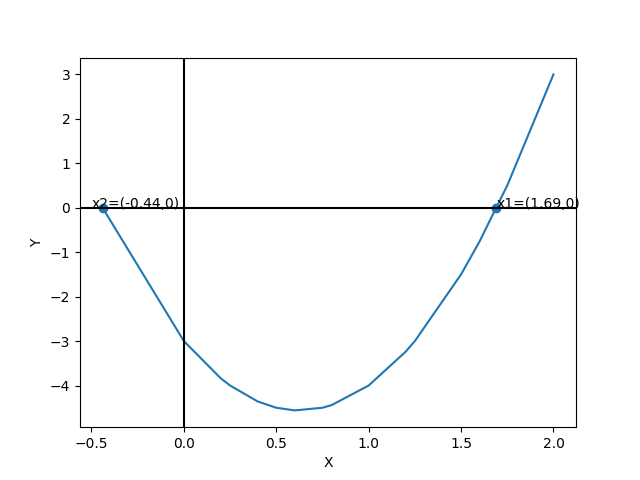
\includegraphics[width=\linewidth]{figplz.png}
\end{figure}

roots upto two decimal places are :-
    
 \begin{enumerate}
     \item 
 \begin{align*} 
x_1 &= \frac{5+\sqrt{(-5)^2-4\times4\times(-3)}}{2\times4}\\ 
&=\frac{5+\sqrt{25+48}}{8}\\ 
&=\frac{5+\sqrt{73}}{8}\\
 &=\frac{5+8.54}{8} \\ 
 &=\frac{13.54}{8}\\ 
 &=1.69 \\ 
\end{align*}
\item
\begin{align*}
x_2 &=\frac{5-\sqrt{(-5)^2-4\times4\times(-3)}}{2\times4}\\ 
&=\frac{5-\sqrt{25+48}}{8}\\ 
&=\frac{5-\sqrt{73}}{8}\\ 
&=\frac{5-8.54}{8} \\ 
&=\frac{-3.54}{8} \\ 
&=-0.44\\
\end{align*}
\end{enumerate}

The roots of the given equation are 1.69 and -0.44
\end{document}













